% results.tex
% Author: Tony Kabilan Okeke
% Date: 2023-03-23

\begin{figure*}[ht]
    \centering
    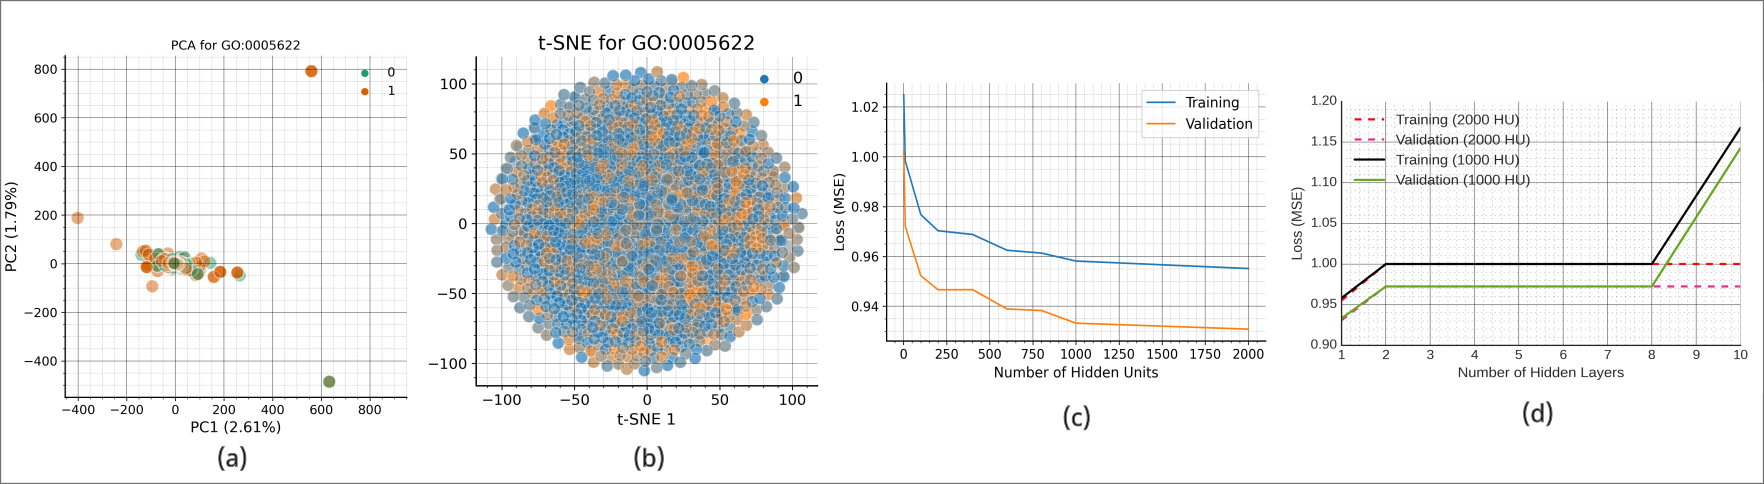
\includegraphics[width=\textwidth]{./images/results.png}
    \captionof{figure}{
        Results from evaluating the autoencoder.
        a) Scatter plot showing first 2 principal components of the data. Explained
        variances shown in axis labels.
        b) Scatter plot showing first 2 t-SNE components of the data.
        c) Autoencoder loss on the validation set with varied number of neurons.
        d) Autoencoder loss on the validation set with varied number of hidden layers.
    }
    \label{fig:results}
\end{figure*}

\section{Results}

First, we performed principal component analysis (PCA) on the logFC values to visualize
the data in a lower-dimensional space. The first two principal components explained
$2.61\%$ and $1.79\%$ of the total variance, respectively. Figure \ref{fig:results}a shows
the scatter plot of the first two principal components. The points are colored by whether
the GO0005622 (the most common GO term) term is enriched or not. No clear separation
between the two classes is observed.

We then visualized the data using t-distributed stochastic neighbor embedding (t-SNE).
Figure \ref{fig:results}b shows the scatter plot of the first two t-SNE components. The
points are colored by whether the GO0005622 term is enriched or not. Again, no clear
separation between the two classes is observed.

Next, we needed to determine the optimal number of neurons and hidden layers for the
autoencoder. To identify the optimal number of neurons, we trained the autoencoder with
varying numbers of neurons in a single hidden layer; we evaluated the model's performance
using the loss on the validation set. We tested the following numbers of neurons: 1, 10,
100, 200, 400, 600, 800, 1000, and 2000. Figure \ref{fig:results}c shows the loss on the
training and validation sets for each number of neurons. The loss on the validation set
decreased as the number of neurons increased, and plateaus at around 2000 neurons.

To identify the optimal number of hidden layers, we trained the autoencoder with varying
numbers of hidden layers. The total number of neurons in the network was first fixed at
2000 (the optimal number of neurons from the previous experiment), and subsequently at
1000. The neurons were distributed so each hidden layer had half the number of neurons
of the previous layer. We tested the following numbers of hidden layers: 1, 2, 3, 4, 5, 6,
7, 8, 9, and 10. Figure \ref{fig:results}d shows the loss on the training and validation
sets for each number of hidden layers. The loss on the validation set increased as the
number of hidden layers increased, with the lowest loss observed at 1 hidden layer.

Finally, we trained the autoencoder with the optimal number of neurons and hidden layers
(2000 neurons in a single hidden layer) over 50 epochs. The performance of the final model
was evaluated using 4-fold cross-validation. The average cross-validation loss was
$0.9632$.
